\section{Temporal Partitioning}

%%%%%%%%%%%%%%%%%%%%%%%%%%%%%%%%%%%%%%%%%

\begin{frame}{Real-Time Systems}

\pause
\begin{block}{Real-Time Constraints from Event to System Response}
\pause
\begin{itemize}[<+->]
    \item Deadlines based on real-time requirements
    \item No deadline misses allowed ever
    \item Prepare for the worst-case
\end{itemize}
\end{block}

\end{frame}


\begin{frame}{Real-Time Systems -- Scheduling Example}

\begin{block}{Task Set}
\begin{tabular}{cccc<{\onslide<3->}c<{\onslide}}
\textbf{Task}&\textbf{Period}&\textbf{Deadline}&\textbf{WCET}&\textbf{ACET}\\ \hline
$T1$&$10$&$5$&$4$&$2$\\
$T2$&$10$&$10$&$6$&$4$
\end{tabular}
\end{block}

\vfill

\includegraphics<2-3>[width=\textwidth]{Figures/real-time-sched-1}
\includegraphics<4>[width=\textwidth]{Figures/real-time-sched-2}

\end{frame}

\begin{frame}{Real-Time Systems -- Pros and Cons}

\begin{block}{}<2->
    \begin{itemize}
        \item<2-> Static guarantees even for the worst-case
        \item<3-> Overprovisioning for the average-case 
    \end{itemize}
\end{block}

\vfill

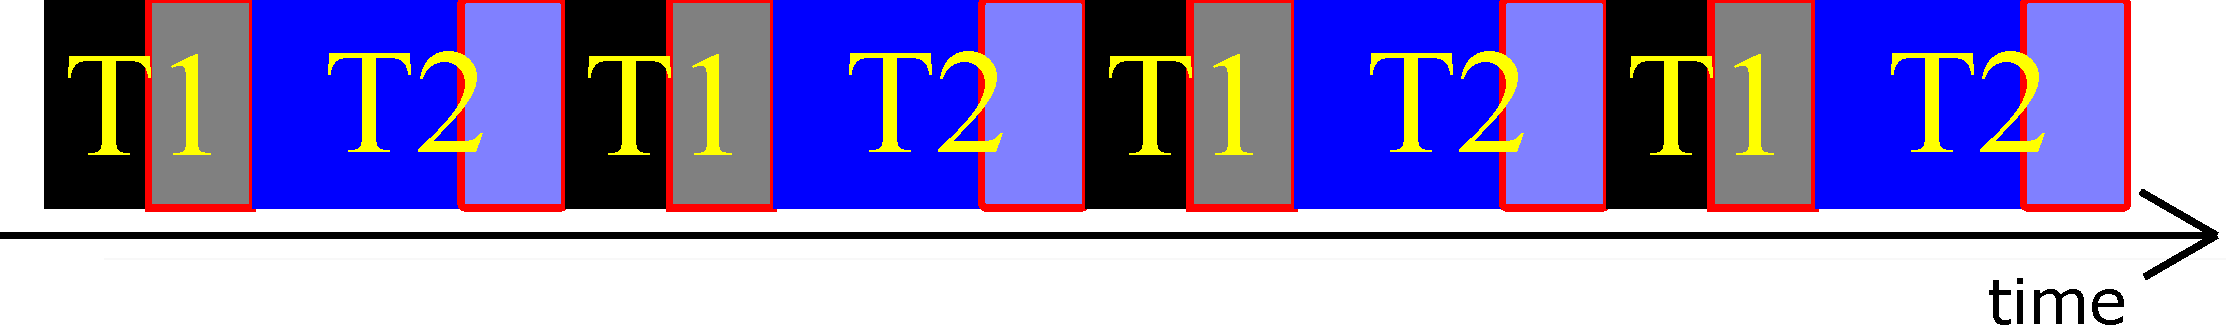
\includegraphics[width=\textwidth]{Figures/real-time-sched-2}

\onslide<4>{\centering \hilightA{Economic need for trading off guarantees for utilization}}

\end{frame}


%%%%%%%%%%%%%%%%%%%%%%%%%%%%%%%%%%%%%%%%%%%%%%%%%%%%%%%%%%%%%%%%%%%%%%%%%%%%%%
\subsection{Full-Scale Mode Switches}

\begin{frame}{Mixed Criticality Levels}

\begin{minipage}{\textwidth}
\begin{block}{Worst-Case Execution Time Estimates}<2->
\begin{itemize}
    \item<3-> Various components are validated against various assumptions
    \item<4-> The stricter assumptions, the longer estimated WCET
\end{itemize}
\end{block}

\begin{block}{Criticality Levels of Tasks}<5->
\begin{itemize}
    \item<6-> Strictness of assumptions
    \item<7-> Ordered set of levels
\end{itemize}
\end{block}
\end{minipage}

\end{frame}

\begin{frame}{Mixed-Criticality Scheduling with Criticality Mode Switches}

\pause
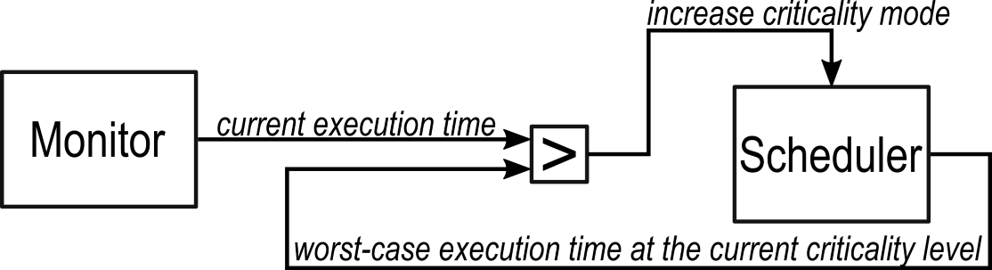
\includegraphics[width=\textwidth]{Figures/mixed-crit-sched-robin}
\pause
\begin{itemize}[<+->]
    \item Start system in the lowest criticality mode
    \item Schedule tasks with criticality not below the current criticality mode
    \item Monitor whether execution violates current assumptions
    \item Switch to higher criticality mode for stricter assumptions
\end{itemize}

\end{frame}


\begin{frame}{Mixed-Criticality Scheduling with Mode Switches}

\only<1-2>{%
\begin{minipage}{\textwidth}
\begin{block}{Task Set $HI$}
\begin{tabular}{cccc}
\textbf{Task}&\textbf{Period}&\textbf{Deadline}&\textbf{WCET}\\ \hline
$T1$&$10$&$5$&$4$\\
$T2$&$10$&$10$&$6$
\end{tabular}
\end{block}

\onslide<2>
\begin{block}{Task Set $LO$}
\begin{tabular}{cccc}
\textbf{Task}&\textbf{Period}&\textbf{Deadline}&\textbf{WCET}\\ \hline
$T1$&$10$&$5$&$2$\\
$T2$&$10$&$10$&$4$\\
$T3$&$10$&$9$&$3$
\end{tabular}
\end{block}
\end{minipage}
}

\only<3->{%
\begin{minipage}{\textwidth}
\begin{block}{Mixed-Criticality Task Set}
\begin{tabular}{ccccc}
\textbf{Task}&\textbf{CL}&\textbf{Period}&\textbf{Deadline}&\textbf{WCET}\\ \hline
$T1$&$HI$&$10$&$5$&$[2,4]$\\
$T2$&$HI$&$10$&$10$&$[4,6]$\\
$T3$&$LO$&$10$&$9$&$[3]$
\end{tabular}
\end{block}

\bigskip

\includegraphics<4>[width=\textwidth]{Figures/mixed-crit-sched-1}
\includegraphics<5>[width=\textwidth]{Figures/mixed-crit-sched-2}
\includegraphics<6>[width=\textwidth]{Figures/mixed-crit-sched-3}
\includegraphics<7>[width=\textwidth]{Figures/mixed-crit-sched-4}

\onslide<6->{\centering \hilightA{Ignoring $LO$ criticality tasks in $HI$ mode}}

\end{minipage}
}

\end{frame}

\begin{frame}{Limitations of Mode Switching Scheduling}

\pause
\begin{block}{Static Verification}\onslide<2->
\begin{itemize}
    \item<3-> Timing guarantees for each mode
    \item<4-> \hilightA{No link to requirements of safety standards}
\end{itemize}
\end{block}

\begin{block}{Runtime Robustness}\onslide<2->
\begin{itemize}
    \item<5-> \hilightA{Ignoring low-criticality tasks}
    \item<6-> \hilightA{Returning to low-criticality mode}
\end{itemize}
\end{block}

\end{frame}


%%%%%%%%%%%%%%%%%%%%%%%%%%%%%%%%%%%%%%%%%%%%%%%%%%%%%%%%%%%%%%%%%%%%%%%%%%%%%%
\subsection{Memory Access Budgeting}

\begin{frame}{Memory Accesses and Execution Time}

\end{frame}

\begin{frame}{Memory Access Budgeting}

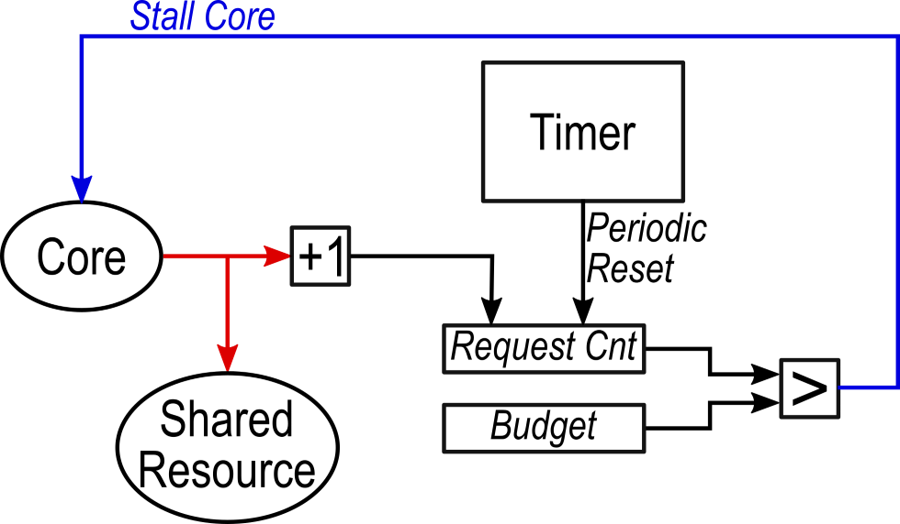
\includegraphics[width=\textwidth]{Figures/budgeting-robin}

\end{frame}


\begin{frame}{Memory Access Budgeting -- Pros and Cons}

\end{frame}

%%%%%%%%%%%%%%%%%%%%%%%%%%%%%%%%%%%%%%%%%%%%%%%%%%%%%%%%%%%%%%%%%%%%%%%%%%%%%%
\subsection{Execution Time Monitoring}

\begin{frame}{Remaining Worst-Case Execution Time}

\end{frame}

\begin{frame}{Execution Time Monitoring}

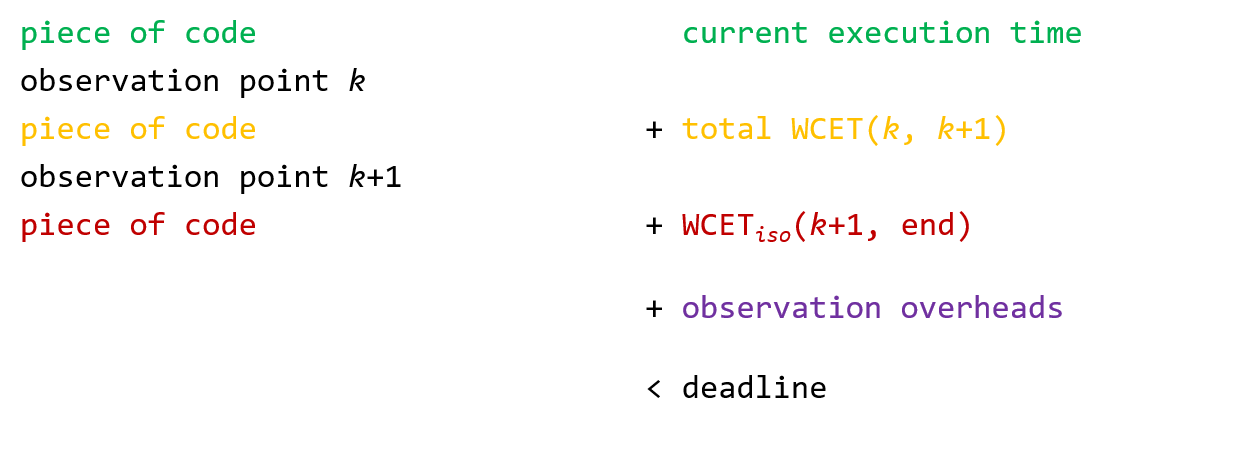
\includegraphics[width=\textwidth]{Figures/exec-time-monitoring-robin}

\end{frame}


\begin{frame}{Execution Time Monitoring -- Pros and Cons}

\end{frame}


%%%%%%%%%%%%%%%%%%%%%%%%%%%%%%%%%%%%%%%%%%%%%%%%%%%%%%%%%%%%%%%%%%%%%%%%%%%%%%
\subsection{Workload Arrival Monitoring}

\begin{frame}{Workload Arrival Functions}

\end{frame}

\begin{frame}{Workload Arrival Monitoring}

\end{frame}


\begin{frame}{Workload Arrival Monitoring -- Pros and Cons}

\end{frame}

%%% Local Variables:
%%% mode: latex
%%% TeX-master: "slides"
%%% End:
